\chapter{Unmanned Aerial Vehicle}
\label{cap:uav}
Con il termine \emph{Unmanned Aerial Vehicle} si intendono velivoli senza pilota, i quali possono essere pilotati da remoto
o possono volare autonomamente secondo un itinerario prestabilito. \\
Gli \ac{UAV} sono attualmente utilizzati per una serie di missioni, incluse le ricognizioni e i ruoli d'attacco; è quindi 
necessaria la distinzione dai missili. Gli \ac{UAV} sono definiti come controllabili, e mantengono un volo orizzontale 
sostenuto e alimentato da un getto o motore alternativo. Un missile può essere considerato come un \ac{UAV}, 
ma si distingue da esso poiché il veicolo è l'arma stessa. \\
La FAA ha racchiuso l'acronimo \ac{UAV} in quello più generale di \ac{UAS} riflettente il 
fatto che questo tipo di veicoli comprende sia sistemi terrestri come gli \ac{UGV} che gli \ac{UAV}. \\
L'utilizzo degli \ac{UAV} oggigiorno è diventato sempre più necessario, nel caso di operazioni militari il loro uso è ormai 
consolidato, mentre è in crescita l'utilizzo per missioni civili e non militari. \\
Il grande vantaggio è il loro impiego in quelle che sono dette missioni \emph{dull, dirty and dangerous} (noiose, sporche e 
pericolose), grazie agli \ac{UAV} infatti è possibile risparmiare risorse economiche ed umane.

\begin{figure}
  \centering
  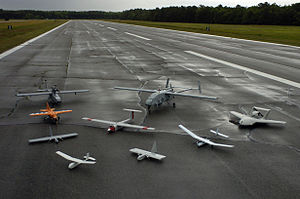
\includegraphics[height=0.25\textheight]{Immagini/gruppouav}
  \caption{Un gruppo di \ac{UAV}}
  \label{img:gruppouav}
\end{figure}

\section{Componenti}
Nonostante il nome faccia pensare ad un dispositivo indipendente, in grado di volare autonomamente, un \ac{UAV} è ben più complesso, 
esso non si riduce al solo velivolo senza pilota, ma anche ad una serie di apparecchiature che permettono il controllo da remoto.
La componentistica di un \ac{UAV} può essere divisa in due: il segmento di volo e il segmento di terra.

\begin{figure}[!h]
  \centering
  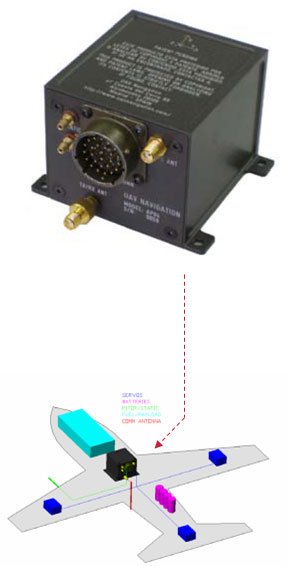
\includegraphics[height=0.25\textheight]{Immagini/segvolo}
  \caption{Componentistica interna di un \ac{UAV}.}
  \label{img:comp}
\end{figure}

\subsection*{Segmento di volo}
La gestione del volo di un \ac{UAV} può variare da modello a modello, alcuni sono in grado di decollare o atterrare autonomamente, altri,
invece, possono essere completamente gestiti da remoto. Il controllo del volo è gestito da remoto o controllato attraverso un percorso
prestabilito. \\
A bordo è presente il \emph{GN\&C} (sistema di Guida, Navigazione e Controllo), che gestisce il volo anche in assenza di segnale da terra,
inoltre a bordo possono essere presenti telecamere che mostrano immagini dall'aeromobile, anche in tempo reale; come nel caso della figura
\ref{img:vista}, l'\ac{UAV} controlla una zona agricola.

\begin{figure}
  \centering
  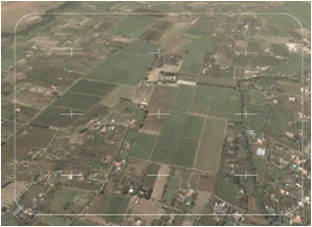
\includegraphics[height=0.25\textheight]{Immagini/segterra3}
  \caption{Vista dalla telecamera di un \ac{UAV}}
  \label{img:vista}
\end{figure}

\subsection*{Segmento di terra}
Il controllo a terra di un \ac{UAV} è costituito da:
\begin{itemize}
 \item GCS: (Ground Control System) È il controllo a terra del velivolo, svolge molte funzioni, come la rilevazione della posizione dell'
 \ac{UAV}, scambio dei dati con il velivolo, permette il pilotaggio manuale e controlla l'orientamento dell'Antenna Tracking System.
 \item Ground Computer: Permette l'elaborazione dei dati di telemetria e delle immagini inviate dall'\ac{UAV} con la telecamera a bordo.
 \item Antenna tracking system: L'uso di questo tipo di apparecchiature permette il controllo del velivolo durante il volo.
 \item Joystick: Questo strumento permette il controllo manuale del velivolo.
\end{itemize}

\begin{figure}[!h]
  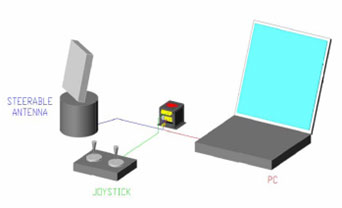
\includegraphics[height=0.25\textheight]{Immagini/segterra1}
  \caption{Apparecchiatura di terra di un \ac{UAV}.}
  \label{img:terra}
\end{figure}

\section{Impieghi tipici degli UAV}
Gli \ac{UAV}, grazie alla possibilità di essere controllati da remoto, si prestano facilmente ad utilizzi di vario tipo. \\

\subsection*{Telerilevamento}
Attraverso il telerilevamento è possibile monitorare e quindi ricavare informazioni, qualitative e quantitative, 
relative all'area coperta dall'\ac{UAV}. \\
Questo tipo di \ac{UAV} utilizza una vasta gamma di sensori come il sensore di misura dello spettro elettromagnetico, 
sensore a raggi gamma, sensori biologici e chimici. I sensori elettromagnetici includono principalmente telecamere a spettro
visivo o a infrarossi (Fig. \ref{img:infrareduav}) come i radar, sono raramente utilizzati anche altri rivelatori di onde 
elettromagnetiche come microonde e sensori spettro ultravioletto.
\begin{figure}[h]
 \centering
 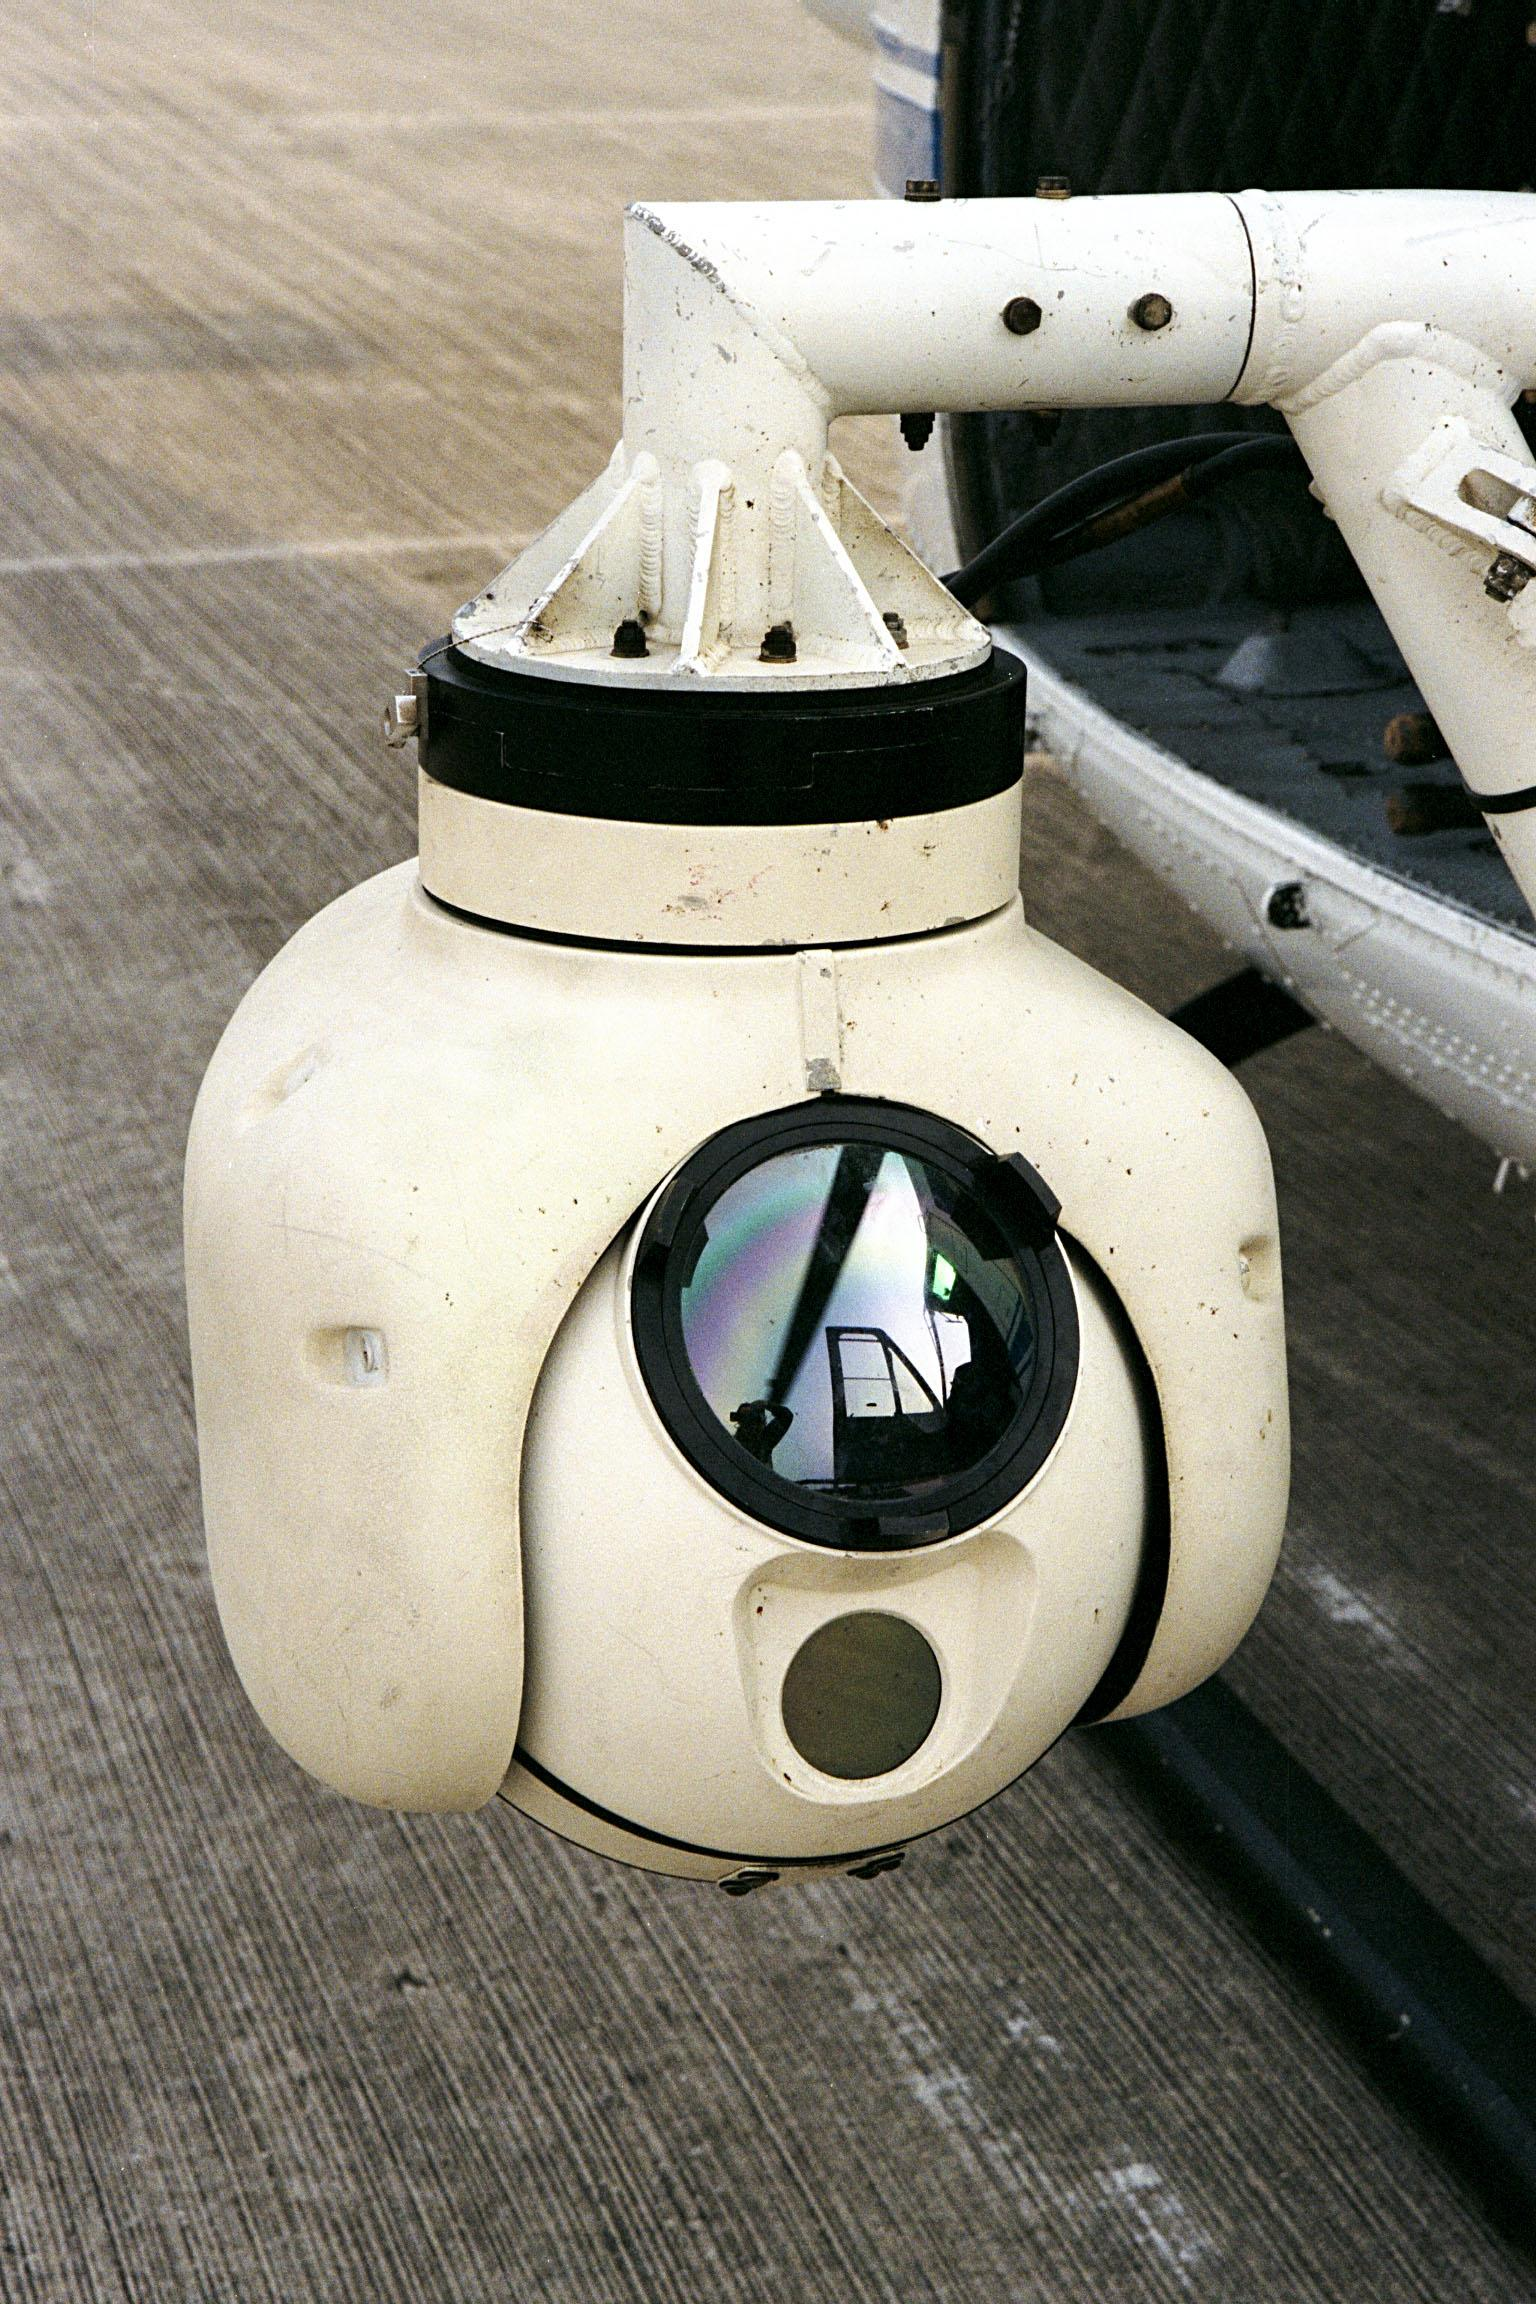
\includegraphics[height=0.5\textwidth]{Immagini/infrareduav}
 \caption{Una fotocamera ad infrarossi montata sul di un \ac{UAV}}
 \label{img:infrareduav}
\end{figure}

I sensori biologici sono sensori in grado di rilevare la presenza di microrganismi nell'aria e vari altri fattori biologici,
mentre i sensori chimici utilizzano spettroscopia laser per analizzare la concentrazione di ciascun elemento in aria.

\subsection*{Sorveglianza Aerea}
Grazie agli \ac{UAV} è possibile sorvegliare vaste aree a basso costo, questo tipo di operazioni comprende: mappatura degli incendi,
monitoraggio del bestiame, sicurezza domestica, stradale e pattugliamento anti-pirateria.
Molto importante è quest'ultimo aspetto, la sicurezza territoriale, delle frontiere e lotta ai narcotrafficanti, infatti nel 2011,
gli Stati Uniti hanno collaborato con il Messico per arginare il fenomeno dell'immigrazione clandestina e del traffico di sostanze 
stupefacenti attraverso il monitoraggio del loro confine

\subsection*{Indagini Geofisiche}
Gli \ac{UAV} sono impiegati anche in indagini geomagnetiche, dove il differenziale del campo magnetico terrestre è utilizzato
per calcolare la struttura della sottostante roccia magnetica, spesso ciò è utile per cercare di predire la posizione di
miniere minerarie e petrolifere.

\subsection*{Trasporto}
Una delle meno comuni funzioni degli \ac{UAV} è quella del trasporto merci. La maggior parte dei carichi utili sono contenuti in un 
vano di carico interno, i carichi esterni invece possono essere legati alla fusoliera o fissati alle ali, in questo caso però ne
risentirà l'aerodinamica, quindi sono spesso racchiusi in un guscio.

\subsection*{Ricerca Scientifica}
Gli \ac{UAV} sono gli unici in grado di penetrare in aree che possono essere troppo pericolose per le imbarcazioni pilotate.
Per esempio la \emph{NOAA} (National Oceanic and Atmospheric Administration), nel 2006 ha iniziato ad utilizzare gli \ac{UAV} come
cacciatori di uragani, questo tipo di aeromobili è in grado di volare all'interno dell'uragano per comunicare quasi in tempo 
reale dati come pressione barometrica standard e dati di temperatura, anche molto vicini alla superficie dell'acqua,
direttamente al National Hurricane Center in Florida. \\ 
Ulteriori applicazioni per aerei senza pilota possono essere quelli del produttore britannico UAVSI, che ha progettato una
variante degli \ac{UAV} particolarmente adatta a climi rigidi, come l'Antartide.

\subsection*{Attacchi Armati}
Gli MQ-1 Predator sono \ac{UAV} armati con missili \ac{HELLFIRE}, 
sempre più utilizzati dagli Stati Uniti come piattaforme per colpire bersagli a terra. I Predators armati sono stati utilizzati 
alla fine del 2001 da basi in Pakistan e Uzbekistan, per lo più volti ad assassinare persone di alto profilo 
(capi terroristi, \dots) in Afghanistan. Da allora, ci sono stati molti casi di attacchi di questo tipo che si svolgono 
in Afghanistan, Pakistan, Yemen e Somalia. Il vantaggio di utilizzare un veicolo senza pilota, 
piuttosto che un aereo con equipaggio, in questi casi è quello di evitare un imbarazzo diplomatico nel caso in cui l'aeromobile 
venisse abbattuto e venissero catturati i piloti, dal momento che i bombardamenti si svolgono in paesi ritenuti cordiali e 
senza il permesso ufficiale di quei paesi.

\subsection*{Ricerca e Salvataggio}
\label{sec:rs}
Un altro ruolo importante per gli \ac{UAV} è quello nelle operazioni di ricerca e soccorso, grazie ad essi, infatti, è possibile
raggiungere agevolmente zone colpite da disastri naturali o causati dall'uomo, per permettere ricognizioni in tempi rapidi. \\
Proprio su un aspetto di questo particolare uso si soffermerà questa tesi: in queste situazioni sarà proprio compito dell'\ac{UAV}
ripristinare le comunicazioni in modo da consentire agli operatori di soccorso di dialogare tra loro, ed eventualmente con 
le persone (civili) coinvolte nella crisi.
\\[1cm]
L'utilizzo degli \ac{UAV} considerato in questa tesi è stato quello del ripristino e gestione delle comunicazioni in aree colpite da crisi 
in cui è molto importante riuscire a mantenere le connessioni attive per facilitare le operazioni di soccorso a seguito di calamità 
naturali o da avvenimenti particolari (terremoti, esondazioni,incidenti stradali, \ldots).

\section{Classificazione}
Gli \ac{UAV}  in genere rientrano in \emph{sei} categorie a seconda della loro funzione, ultimamente però i ruoli svolti raccolgono più
di una sola funzione in un solo aeromobile:

\begin{description}
 \item[Target and decoy] Fanno da obiettivo aereo o terrestre simulando un aeromobile o un missile nemico.
 \item[Reconnaissance] Forniscono informazioni sul campo di battaglia.
 \item[Combat] Hanno la capacità di attaccare in missioni ad alto rischio.
 \item[Logistics] \ac{UAV} specificamente progettato per il carico e la gestione della logistica.
 \item[Research and development] Utilizzati per sviluppare ulteriormente le tecnologie \ac{UAV}.
 \item[Civil and Commercial UAVs] \ac{UAV} sviluppati principalmente per applicazioni civili e commerciali.
\end{description}

È possibile un altro tipo di classificazione in termini di altitudine/range:

\begin{description}
 \item[Handheld] (altitudine di circa 600 m), circa 2 km di range.
 \item[Close] (altitudine massima 1500 m), più di 10 km di range.
 \item[NATO type] (massima altitudine 3000 m) più di 50 km di range.
 \item[Tactical] (altitudine di circa 5500 m), circa 160 km di range.
 \item[MALE] (altitudine media, lunga durata) altitudine oltre 9000 m, più di 200 km di range. 
 \item[HALE] (elevata altitudine, lunga durata) altitudine oltre 9100 m, range indefinito.
 \item[HYPERSONIC] (alta velocità, supersonico (Mach 1–5) o ipersonico (Mach 5+)) altitudine di circa 15200 m (sub-orbitale) e range oltre 200 km.
\end{description}

\section{Eventi civili che hanno coinvolto UAV}
Come già detto nell'introduzione, il vantaggio che deriva dall'utilizzo degli \ac{UAV} è l'utilizzo nelle missioni 
\emph{dull, dirty and dangerous}, negli ultimi anni ci sono state varie occasioni che hanno coinvolto gli \ac{UAV}:
\begin{itemize}
 \item Un importante coinvolgimento non bellico degli \ac{UAV} è stato durante il terremoto del Tohoku del 2011. I velivoli americani 
 \emph{Global Hawk} hanno sorvolato la Centrale nucleare di Fukushima Dai-ichi, in Giappone, per poter addentrarsi nelle zone vietate per
 le forti radiazioni. Lo scopo principale è stato quello di controllare i reattori dopo le esplosioni causate dal forte sisma.
 \item In Italia un recente utilizzo degli \ac{UAV} è stato durante il recente terremoto in \emph{Emilia}, sono stati utilizzati alcuni 
 velivoli per controllare le aree inaccessibili a causa delle macerie.
\end{itemize}
